% --- Program Section ---

\newprogram{Program 14}{Implement solveNQueens(n: int) -> List[List[str]] function taking board dimension and
returning all valid board layout configurations. }
\subsection*{Code}


\begin{lstlisting}[language=python]
from typing import List


def solveNQueens(n: int) -> List[List[str]]:
    result = []

    board = [["."] * n for _ in range(n)]

    columns = set()
    diagonals = set()
    anti_diagonals = set()

    def backtrack(row):
        # All queens placed
        if row == n:
            result.append(["".join(row) for row in board])
            return

        for col in range(n):

            # Check if column or diagonal is already occupied
            if col in columns:
                continue

            if row - col in diagonals:
                continue

            if row + col in anti_diagonals:
                continue

            # Place queen
            board[row][col] = "Q"
            columns.add(col)
            diagonals.add(row - col)
            anti_diagonals.add(row + col)

            # Move to next row
            backtrack(row + 1)

            # Remove queen (backtrack)
            board[row][col] = "."
            columns.remove(col)
            diagonals.remove(row - col)
            anti_diagonals.remove(row + col)

    backtrack(0)

    return result


# Example
n = 4

solutions = solveNQueens(n)

print("Number of solutions:", len(solutions))

for solution in solutions:
    for row in solution:
        print(row)
    print()
\end{lstlisting}

\subsection*{Output}
\begin{center}
    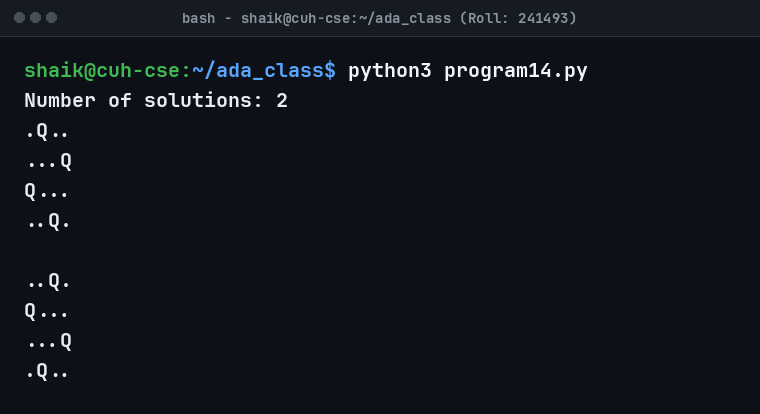
\includegraphics[width=0.88\textwidth]{Images/output_screenshot14.png}
\end{center}

\subsection*{GitHub Scan Code}
\begin{center}
    \begin{minipage}{0.3\textwidth}
        \centering
        % Generates a 2.5cm high QR code directly linking to the code file
        \qrcode[height=3.5cm]{https://github.com/gytdrop/ada_class/blob/main/program14.py} \\[0.2cm]
        \scriptsize\ttfamily Scan to view source code 
    \end{minipage}
\end{center}


% Add a horizontal line that indicates the END of the program.
\vspace{1cm}
\begin{center}
    \rule{1\textwidth}{1pt} % Clean, centered 1pt thick horizontal line
\end{center}